\documentclass[pdf]{beamer}
\usepackage[utf8]{inputenc}
\usepackage{bookman}
\usetheme{Madrid}

\usepackage{xcolor}
\definecolor{light-gray}{gray}{0.95}
\newcommand{\code}[1]{\colorbox{light-gray}{\texttt{#1}}}
\newcommand{\mono}[1]{\texttt{#1}}


\mode<presentation>{}
%% preamble
\title{Tools and tips}
\subtitle{Notes worth remembering}
\author{Fernando}
%%\email{}
\institute{\href{https://github.com/fgrando}{\emph{my github}}}
\date{\today} 

\begin{document}

%% title frame
\begin{frame}
    \titlepage
\end{frame}


\begin{frame}{Motivation}
    I create this file to keep track of interesting tools and some tips learned
    along the way.\\
    And also to learn \LaTeX  beamer \mono{:)}
\end{frame}


\begin{frame}
  \frametitle{silversearcher-ag}
  \code{ag} is like grep or ack. Very useful for searching terms in documentation and code.
  
  Installation:
  \begin{itemize}
    \item Linux: \mono{apt install silversearcher-ag}
    \item Windows: \url{https://blog.kowalczyk.info/software/the-silver-searcher-for-windows.html}
  \end{itemize}
  
  \begin{figure}
    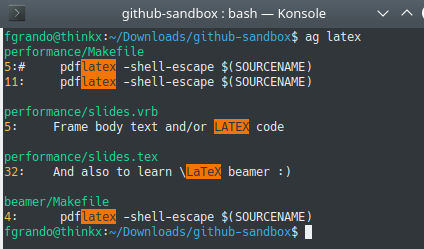
\includegraphics[scale=0.4]{data/ag-terminal-linuxpng.png}
    %\caption{console execution}
  \end{figure}
  %Windows port: \href{https://blog.kowalczyk.info/software/the-silver-searcher-for-windows.html}{\beamergotobutton{Link}}
  

\end{frame}


\begin{frame}
  \frametitle{PDF to Text}
  Extract text from PDF files.
  TODO
\end{frame}


\begin{frame}
  \frametitle{From SVN to GIT}
  Useful commands:
  \begin{itemize}
    \item \mono{svn commit -m "first commit"}
      \begin{itemize}
      \item \mono{git commit -m "first commit"}
      \end{itemize}
    
    \item \mono{svn revert <file>}
      \begin{itemize}
      \item \mono{git checkout <file>}
      \end{itemize}
    \end{itemize}

\end{frame}




\end{document}
